\documentclass[xcolor=dvipsnames]{beamer}

\usecolortheme[RGB={107,142,35}]{structure}
\usepackage{beamerthemesplit}
\usepackage{graphicx}
\usepackage[francais]{babel}
\usepackage[utf8]{inputenc} 

\title{Interrogation en langue naturelle}
\subtitle{Projet M1}
\author{Ludovic Bonnefoy \and Romain Deveaud}
\date{Jeudi 18 juin 2009}
\institute{Tutoré par Marc El-Bèze et encadré par Eric Charton}

\begin{document}

\frame{\titlepage}

\section{Présentation de la problèmatique}
\begin{frame}
\begin{block}{\Large{Présentation de la problèmatique}}
\tiny{Définition, bref état de l'art, objectifs du projet...}
\end{block}
\end{frame}
\subsection{Définition}
\frame
{
  \frametitle{Définition}
  \begin{itemize}
    \item<1-> Que signifie interrogation en langue naturelle?
    \item<2-> Permettre à un utilisateur de questionner un outil de recherche d'information avec des requêtes formulées en langue naturelle.
    \item<3-> Enjeu majeur : interpréter la question et comprendre le type de réponse attendu par l'utilisateur.
  \end{itemize}
}
\subsection{Un domaine de recherche en plein essort}
\frame
{
    \frametitle{Un domaine de recherche en plein essort}
    \begin{itemize}
        \item<1-> Moteurs de recherche intégrant les requêtes en langue naturelle
        \item<2-> Google
        \begin{figure}
            \includegraphics[scale=0.35]{google}
        \end{figure}
        \item<3-> Powerset
        \begin{figure}
            \includegraphics[scale=0.30]{powerset}
        \end{figure}
    \end{itemize}
}
\subsection{Objectifs du projet}
\frame
{
    \frametitle{Objectifs du projet}
    \begin{itemize}
        \item<1-> Nous n'avons pas à réaliser un moteur complet.
        \item<2-> Nous devons passer d'une requête en langage naturel à un ensemble d'éléments permettant d'interroger des moteurs existant.
        \item<3-> Interface avec NLGbAse, système comprenant plusieurs outils d'extraction d'informations.
    \end{itemize}
}
\subsection{Présentation de NLGbAse}
\frame
{
    \frametitle{Présentation de NLGbAse}
    \begin{itemize}
        \item<1-> Une ressource ontologique basé sur un corpus documentaire Wikipédia.
        \item<2-> Associe à chaque fiche Wikipédia une classe. \\
            Ex : Molière \texttt{=>} pers ; Avignon \texttt{=>} loc
        \item<3-> Trois moteurs de recherche d'information permettant d'interroger l'ontologie.
    \end{itemize}
}
\frame
{
    \frametitle{Outils d'extraction d'informations proposés par NLGbAse}
    \begin{itemize}
        \item<1-> Moteur classique utilisant la similarité cosinus
        \item<2-> Moteur utilisant la similarité cosinus et proposant de filtrer les résutats par une classe \\
                Ex : Je cherche les entreprises faisant des recherches sur les moteurs en langage naturel \\
                mots clés : recherches moteurs langage naturel ; filtre : org
   \end{itemize}
    \begin{figure}
        \includegraphics[scale=0.60]{similarite_cosine}
    \end{figure}

}
\frame
{
    \frametitle{Outils d'extraction d'informations proposés par NLGbAse}
    \begin{itemize}
        \item<1-> Moteur utilisant un score de compacité. \\
               Ne retourne pas une liste de documents mais la réponse exacte. \\
               Nécessite trois informations : l'entité cible, les mots près desquels peut se trouver la réponse (attracteurs) et la classe de la réponse.\\
               Ex : Quand est né Victor Hugo? \\
               On va rechercher dans la fiche de l'entité cible Victor Hugo une date près du mot \og{}né\fg{}.
    \begin{figure}
        \includegraphics[scale=0.60]{compacite}
     \end{figure}
   \end{itemize}
}
 
\subsection{Formalisation du problème}
\frame 
{
    \frametitle{Formalisation du problème}
    \begin{itemize}
        \item<1-> L'objectif de notre projet est d'obtenir à partir d'une requête formulée en langage naturel toutes les éléments nécessaire pour interroger l'ontologie proposée par NLGbAse par l'intermédiaire des moteurs à notre disposition.
        \item<2-> Deux tâches principales :
        \item<3-> Identifier les mots porteurs de sens et les entités cibles.
        \item<4-> Déterminer la classe de la réponse attendue.
    \end{itemize}
}

\section{Méthodes déployées}
\begin{frame}
\begin{block}{\Large{Méthodes déployées}}
\tiny{Analyse de la question, identification des classes, sélection des mots porteurs de sens}
\end{block}
\end{frame}
\subsection{Pré-requis}
\frame
{
    \frametitle{Pré-requis}
    \begin{itemize}
        \item<1-> Obtenir la structure de la requête, identifier les éléments qui la compose.
        \item<2-> Comment?
        \item<3-> Utilisation d'un Analyseur Morpho-Syntaxique qui permet de mettre en évidence la structure d'un texte.
    \end{itemize}
}
\frame
{
    \frametitle{LinkGrammar}
    \begin{itemize}
        \item  Who is Black Sabbath's singer?
    \end{itemize}
    \begin{figure}
        \includegraphics[scale=0.60]{linkgrammar}
    \end{figure}
}

\subsection{Tâche 1 : identifier la classe de la réponse attendue}
\frame
{
    \frametitle{A l'aide de règles}
    \begin{itemize}
        \item<1-> Règles portant sur les pronoms interrogatifs.
        \item<2-> Who \texttt{=>} pers
        \item<3-> How much \texttt{=>} amount
        \item<4-> What day \texttt{=>} date
        \item<5-> ...
    \end{itemize}
}

\frame
{
    \frametitle{Trouver la classe à partir de l'objet de la question}
    \begin{itemize}
        \item<1-> Si l'objet de la question est une entité nommée alors on cherche sa classe. \\
        \item<2-> Pour cela on utilise l'ontologie NLGbAse.
        \item<3-> Ex : What is a 2CV?
        \item<4-> Si l'objet est un nom commun on utilise les hypéronymes donnés par WordNet.
    \end{itemize}
}

\frame 
{
    \frametitle{WordNet}
    \begin{itemize}
        \item<1-> Wordnet est une base de donnée lexicale.
        \item<2-> Classe tout les mots dans un arbre d'hypéronymes.
        \item<3-> Nous avons associé des classes à un certains nombres de mots de haut niveau dans cet arbre.
    \end{itemize}
    \begin{figure}
        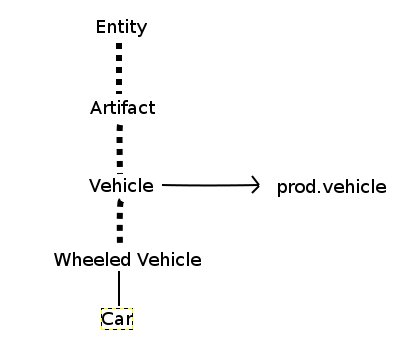
\includegraphics[scale=0.30]{wordnet}
        \caption{Ex : What is Gaston Lagaffe's car? \texttt{=>} prod}
    \end{figure}
}

\subsection{Tâche 2 : sélection d'attracteurs pour le calcul de la compacité}
\frame
{
    \frametitle{Sélection d'attracteurs pour le calcul de la compacité}
    \begin{itemize}
        \item<1-> L'objet de la question est exclu car il est utilisé comme entité source.
        \item<2-> Mots à valeur sémantique forte. \\
            Utilisation combinée des étiquettes de l'analyseur syntaxique et d'un anti-dictionnaire.
        \item<3-> Problème : Qui est la femme de Napoléon?\\
            Interessant de choisir épouse comme attracteur.
        \item<4-> Les synonymes donnés par Wordnet.
    \end{itemize}
}

\section{Expériences et résultats}
\begin{frame}
\begin{block}{\Large{Expériences et résultats}}
\tiny{Evaluation de notre système, formalisme de test utilisé, résultats obtenus}
\end{block}
\end{frame}
\subsection{Evaluation de notre système}
\frame
{
  \frametitle{Evaluation de notre système}
  \begin{itemize}
    \item<1-> Pourquoi une évaluation?
    \item<2-> Mesures des performances.
    \item<3-> Comparaison avec les autres systèmes existants.
    \item<4-> Qu'est-ce qu'on évalue?
    \item<5-> Capacité du système à transformer une requête formulée en langage naturel en données compatible avec des extracteurs d'informations.
    \item<5-> Attribution correcte de la classe de la réponse attendue.
    \item<6-> Bonne sélection des mots porteurs de sens.
  \end{itemize}
}
\subsection{Corpus d'évaluation}
\frame
{
  \frametitle{Corpus d'évaluation (1)}
  \begin{itemize}
    \item<1-> Utilisation d'un corpus issu d'une conférence de traitement automatique de la lange naturelle : Question-Answer de TREC12 (500 questions formulées en langage naturel).
    \item<2-> $<top>$\\
$<num> Number: 1919$\\
$<type> Type: factoid$\\
$<desc> Description:$\\
$How \: big \: is \: Mars?$\\
$<resp> Responses:$\\
$1.7 \: million \: kilometers$\\
$millions \: of \: miles$\\
$...$\\
$</top>$
  \end{itemize}
}
\frame
{
  \frametitle{Corpus d'évaluation (2)}
  \begin{itemize}
    \item<1-> Création d'un nouveau formalisme adapté à l'évaluation de notre système.
    \item<2-> $How \: big \: is \: Mars?$\\
    $cible \: : \: Mars$\\
    $classe \: de \: la \: cible \: : \: loc$\\
    $attracteurs \: : \: big;large$\\
    $classe \: de \: la \: r\acute{e}ponse \: attendue \: : \: amount$
    \item<3-> Etiquetage des 500 questions \og{}à la main\fg{}. 
  \end{itemize}
}
\subsection{Standards de mesures}
\frame
{
  \frametitle{Standards de mesures}
  \begin{itemize}
    \item<1-> $Pr\acute{e}cision_i = \frac{nombre \: d'attributions \: correctes \: de \: la \: classe \: i}{nombre \: d'attributions \: de \: la \: classe \: i}$
    \item<2-> $Rappel_i = \frac{nombre \: d'attributions \: correctes \: de \: la \: classe \: i}{nombre \: de \: questions \: \acute{e}tiquet\acute{e}es \: comme \: appartenant \: \grave{a} \: la \: classe \: i}$
    \item<3-> $F-Score_i = 2 \: \times \: \frac{Pr\acute{e}cision_i \: \cdot \: Rappel_i}{Pr\acute{e}cision_i \: + \: Rappel_i}$
  \end{itemize}
}
\subsection{Résultats}
\frame
{
    \frametitle{Capacité d'attribution des classes de réponses attendues}
    \begin{table}[h]
        \begin{center}
            \begin{tabular}{|p{2.5cm}|l|l|l|}
                \hline
                Catégorie & (\={p}) & (\={r}) & (\={F}-s) \\
                \hline
                Pers & 0.81 & 0.81 & \textbf{0.81} \\
                \hline
                Org & 0.64 & 0.61 & \textbf{0.63} \\
                \hline
                Loc & 0.76 & 0.77 & \textbf{0.76} \\
                \hline
                Date & 0.91 & 0.98 & \textbf{0.95} \\
                \hline
                Amount & 0.99 & 0.92 & \textbf{0.92} \\
                \hline
                Unk & 0.69 & 0.64 & \textbf{0.66} \\
                \hline
                \hline
                Total & 0.80 & 0.78 & \textbf{0.79} \\
                \hline
            \end{tabular}
            \caption{Précision (\={p}), Rappel (\={r}), F-Score (\={F}-s) obtenus sur le corpus QA de TREC 12}
        \end{center}
    \end{table}
}
\frame
{
    \frametitle{Capacité de sélection des mots porteurs de sens}
    \begin{table}[htbp]
        \begin{center}
            \begin{tabular}{|p{8cm}|l|}
                \hline
                Type de mots-clés & (S(C)) \\
                \hline
                Mots-clés extraits pour une recherche par similarité cosinus & \textbf{54.03\%} \\
                \hline
                Entités nommées extraites pour une recherche de type question-réponse (compacité) & \textbf{66.23\%} \\
                \hline
                Mots-clés extraits pour une recherche de type question-réponse (compacité) & \textbf{73.28\%} \\
                \hline
            \end{tabular}
            \caption{Satisfaction (S(C)) obtenue sur le corpus de test}
        \end{center}
    \end{table}
}
\section{Conclusions et perspectives}
\begin{frame}
\begin{block}{\Large{Conclusions et perspectives}}
\tiny{Travail effectué, autres réalisations, bilan du projet}
\end{block}
\end{frame}
\subsection{Retour sur le travail effectué}
\frame
{
  \frametitle{Retour sur le travail effectué}
  \begin{itemize}
    \item<1-> Recherche et documentation sur le domaine du Traitement Automatique de la Langue Naturelle et de la Recherche d'Information.
    \item<2-> Développement d'un système permettant l'interrogation de systèmes de recherche d'informations par des questions formulées en langage naturel.
    \item<3-> Création d'un corpus d'évaluation complet en libre téléchargement.
    \item<4-> Evaluation du système et production de résultats proches de l'état de l'art.
  \end{itemize}
}
\subsection{Mais encore...}
\frame
{
  \frametitle{Mais encore...}
  \begin{itemize}
    \item<1-> Rédaction et soumission d'un article scientifique pour une convention jeunes chercheurs : MajecStic.
    \item<2-> Mise en place d'une version en ligne de notre système par le biais d'un script CGI.
    \item<3-> Création d'un script d'installation permettant le déploiement rapide sur une nouvelle machine.
    \item<4-> Gestion du projet et des sources avec GoogleCode et SubVersion.
  \end{itemize}
}
\subsection{Pour finir}
\frame
{
  \frametitle{Pour finir} 
  \begin{itemize}
      \item<1-> Système expérimental mais fonctionnel.
      \item<2-> Apport d'une solution originale pour l'interrogation de moteurs de recherche en langage naturel.
      \item<3-> Projet enrichissant qui nous a fait découvrir des perspectives de recherche intéressantes.
      \item<4-> Merci de votre attention, voici maintenant la démonstration.
  \end{itemize}
}

\end{document}
